\chapter{Methodology and data Gathering}
\label{chapter:methodology}
This thesis will be focused mainly on classification problem of the “human presence” i.e. if the human is present or not. This will be a supervised learning problem where the features will be mapped to the classes/labels.
For this thesis, we are using VTT built 25 GHz radar along with Raspberry pi. The methodology includes Data collection, Data cleaning, Model Building and Model deployment. Here is a flow, how the process will be conducted in the upcoming months.

\begin{figure}[ht]
  \begin{center}
    % below the size of the figure has been reduced for example
    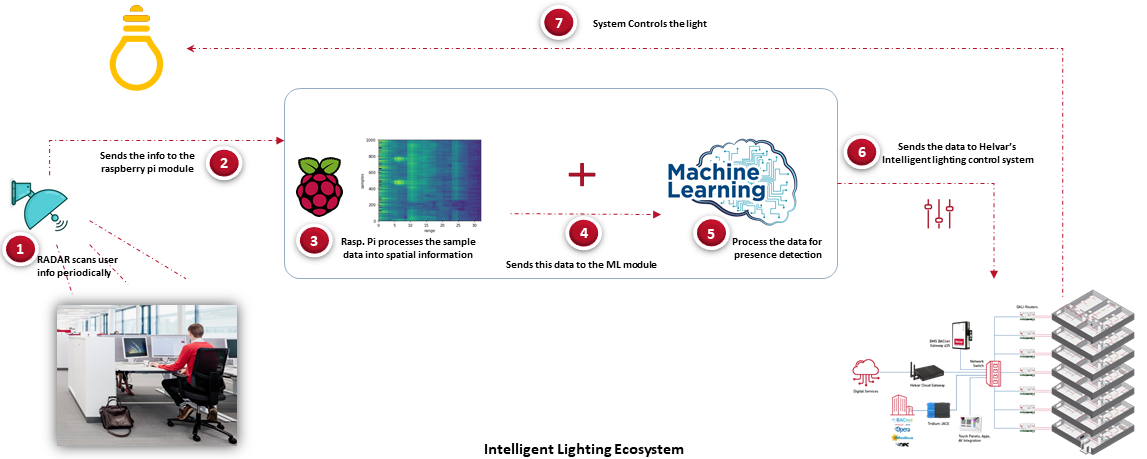
\includegraphics[width=1\textwidth]{Master's thesis/images/thesis_presentation.png} 
    \caption{Overall Process}
    \label{fig:basic_principle}
  \end{center}
\end{figure}


\begin{enumerate}
    \item Radar provides Analog to Digital converted signal. However, this information is not sufficient to distinguish between human presence or absence. Therefore, in order to detect human presence i.e. to collect the labels for the data, we will be using RGB camera for the purpose of creating ground truth. Radar data will be mapped with RGB presence detection based on each time frame.
    \item The data obtained will be feature engineered using multiple techniques.
    \item The idea is engineer the received radar signal of every time frame to a 2-D map and then treating this 2-D map as an image or set of features.
    \item Deep Neural Networks or other Machine Learning techniques will be applied on this already processed data.
    \item For the purpose of training, we will leverage the cloud resources by AWS.
    \item The last step is to deploy these models on the edge devices.
\end{enumerate}

The ultimate objective is to create a more sustainable lighting control solution. Currently at Helvar, the most effective control system turns off the luminaires after 10 min of human absence. Even if, we are able to bring down these power wasteful windows by 50pc, it would make huge impact on the society. Not only it will contribute to sustainability but will also result in lower power consumption and therefore less electricity bills. Lastly, it will add a lot of business value to Helvar as a company.





The Radar set to receive signals for the interval of 16.7ms. This means in one second, an approximate of 60 signals are generated. The radar data is collected for multiple days in a meeting room of Helvar’s headquarters in Espoo. This means on average, the radar generated 60*60*60*24 samples in 1 day. In an ever-moving environment like IT offices, its almost impossible to annotate such vast amount of data manually. It’s not possible to label if a person was present or not for every second for the radar data manually.  One approach was to label the data using the meeting calendars i.e. label the data True if the meeting room is booked. But this approach is highly prone to false labelling. For an example, a meeting room can be occupied by a person even if its not booked. On the other hand, it may be possible that no one comes to the meeting the meeting room despite the booking. Therefore, the more reliable labelling mechanism was desired.

\section{Ground truth with RGB camera}
\label{section:environments}
The data which is used in this thesis is hours and hours of data. In order to achieve reliable inference from our data, precise labelling is required for the training set. Therefore, for creating the labels for the Radar data for training set, an RGB camera is used. 
With the advancement of Machine Learning and Deep Learning libraries, object detection and object recognition can be done with accuracy as high as 100%. Some more lines about CV
The RGB camera and Radar are mounted next to each other, so that the field of view of Radar and camera overlaps. For the purpose of labelling the Radar data, the scene is captured with an RGB camera alongside Radar. The camera is connected to a 32-bit Raspberry pi 4 which dumps the data periodically the video data periodically after 1 sec. The camera used in this thesis captures 60 frames per second (fps).
Once the data is dumped, the data is cleaned and pushed to an object detection deep learning model. For this project Yolov3 is used for object detection. YOLOv3 is extremely fast and accurate. In mAP measured at .5 IOU YOLOv3 is on par with Focal Loss but about 4x faster. YOLOv3 uses a few tricks to improve training and increase performance, including multi-scale predictions, a better backbone classifier, and more. 
(https://pjreddie.com/darknet/yolo/)
Once the data is cleaned into AWS, yolov3 is run on the RGB data collected. Every second of collected data contains 60 frames, so for every second YOLOv3 generates 60 labels. In the Lighting industry, the requirement for getting the true labels is within few seconds. The accuracy of milliseconds is not required in lighting industry. Therefore, for the sake of simplicity and better results, the mode value of the 60 labels was taken for every second. 

Specification of camera in more detail

After using this pipeline, the labels corresponding to every second of Radar data is ready.
Its worth noticing that there might be some inaccuracies in the labelling because of the difference in the angle of view. For instance, the Radar has a centre angle of 210 degrees, whereas camera operates within 180 degrees.


\section{Data Pipeline}
\label{section:environments}
For Radar Data
For RGB Data
For PIR Data


\section{Feature Extraction}
\label{section:environments}


